

\section{Analýza Priepustnosti Lyžiarskeho Strediska}
\subsection{Výsledky Experimentu}

Na základe poskytnutých simulácií boli vyhodnotené priepustnosti rôznych zariadení v lyžiarskom stredisku.
Simulácia odhalila kritické body,kde dôjde k akumulácii návštevníkov, čo môže viesť k predĺženiu čakacích časov a zníženiu celkovej spokojnosti.

\subsection{Priepustnosť a Obslužné Doby}
\begin{itemize}
  \item Pokladna1 a Pokladna2 ukázali podobné priemerné využitie, s maximálnymi dĺžkami radu dosahujúcimi 27 a 26 návštevníkov v najvrcholnejších hodinách sezóny.
  \item PokladnaAutomat mala nižšie využitie a kratšie čakacie doby, čo naznačuje lepšiu efektivitu oproti tradičným pokladniam.
  \item Cafeteria bar vykázala najvyššie využitie s výrazne dlhšími čakacími dobami, čo poukazuje na potrebu zlepšenia v tejto oblasti.
\end{itemize}

\subsection{Záver}
Optimalizácia procesov v lyžiarskom stredisku, najmä zvýšenie priepustnosti v oblastiach s vysokým využitím, by mohla mať významný dopad na zlepšenie plynulosti prevádzky a návštevníckej skúsenosti. Zdá sa, že automatizované pokladne by mohli prispieť k zvýšeniu rýchlosti obsluhy a zníženiu čakacích dôb, čo je jeden z možných smerov k zlepšeniu.


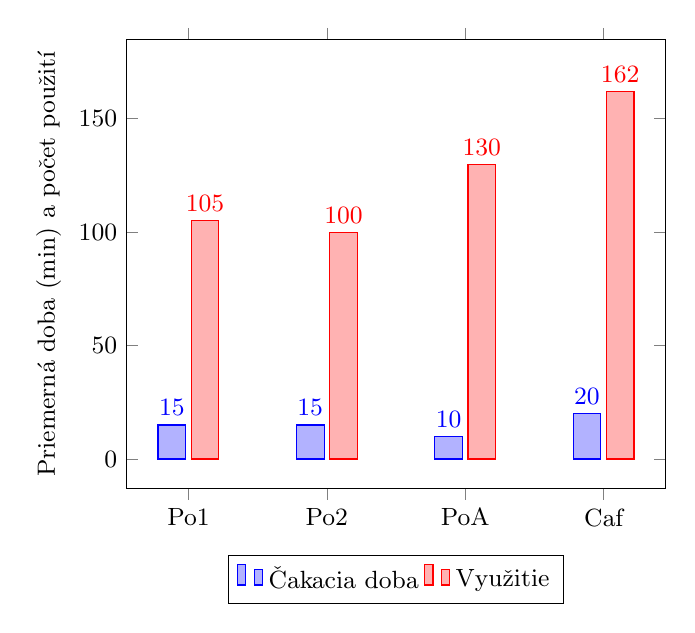
\begin{tikzpicture}\small
    \begin{axis}[
        ybar,
        enlargelimits=0.15,
        ylabel style={font=\small},
        xlabel style={font=\small},
        legend style={at={(0.5,-0.15)},
        anchor=north,legend columns=-1},
        ylabel={Priemerná doba (min) a počet použití},
        symbolic x coords={Po1,Po2,PoA,Caf},
        xtick=data,
        nodes near coords,
        nodes near coords align={vertical},
        ]
    \addplot coordinates {(Po1,15) (Po2,15)
      (PoA,10) (Caf,20)};
    \addplot coordinates {(Po1,105) (Po2,100)
      (PoA,130) (Caf,162)};
    \legend{Čakacia doba, Využitie}
    \end{axis}
\end{tikzpicture}
